\documentclass[margin=1mm]{standalone}

\usepackage{times}
\usepackage{tikz}
\usepackage{pgfplots}
\usepackage{siunitx}
\usetikzlibrary{calc, tikzmark, shapes, shapes.arrows, arrows, 3d, positioning}
\pgfplotsset{compat=1.17}

% \definecolor{llnlblue}{HTML}{003262} % berkeley
\definecolor{llnlblue}{RGB}{255,255,255}
% \definecolor{llnlblue}{HTML}{0b62ad} % lanl
% \definecolor{llnlblue}{HTML}{3B7EA1}
% \definecolor{calgold}{HTML}{FDB515} % berkeley
\definecolor{calgold}{RGB}{200,200,200} % berkeley
% \definecolor{calgold}{HTML}{FFC61E} % lanl
% \definecolor{founder}{HTML}{3B7EA1}
\definecolor{founder}{RGB}{0,0,0}
\definecolor{medalist}{HTML}{C4820E}
\definecolor{goldengate}{HTML}{ED4E33}
\definecolor{ion}{HTML}{CFDD45}

\begin{document}
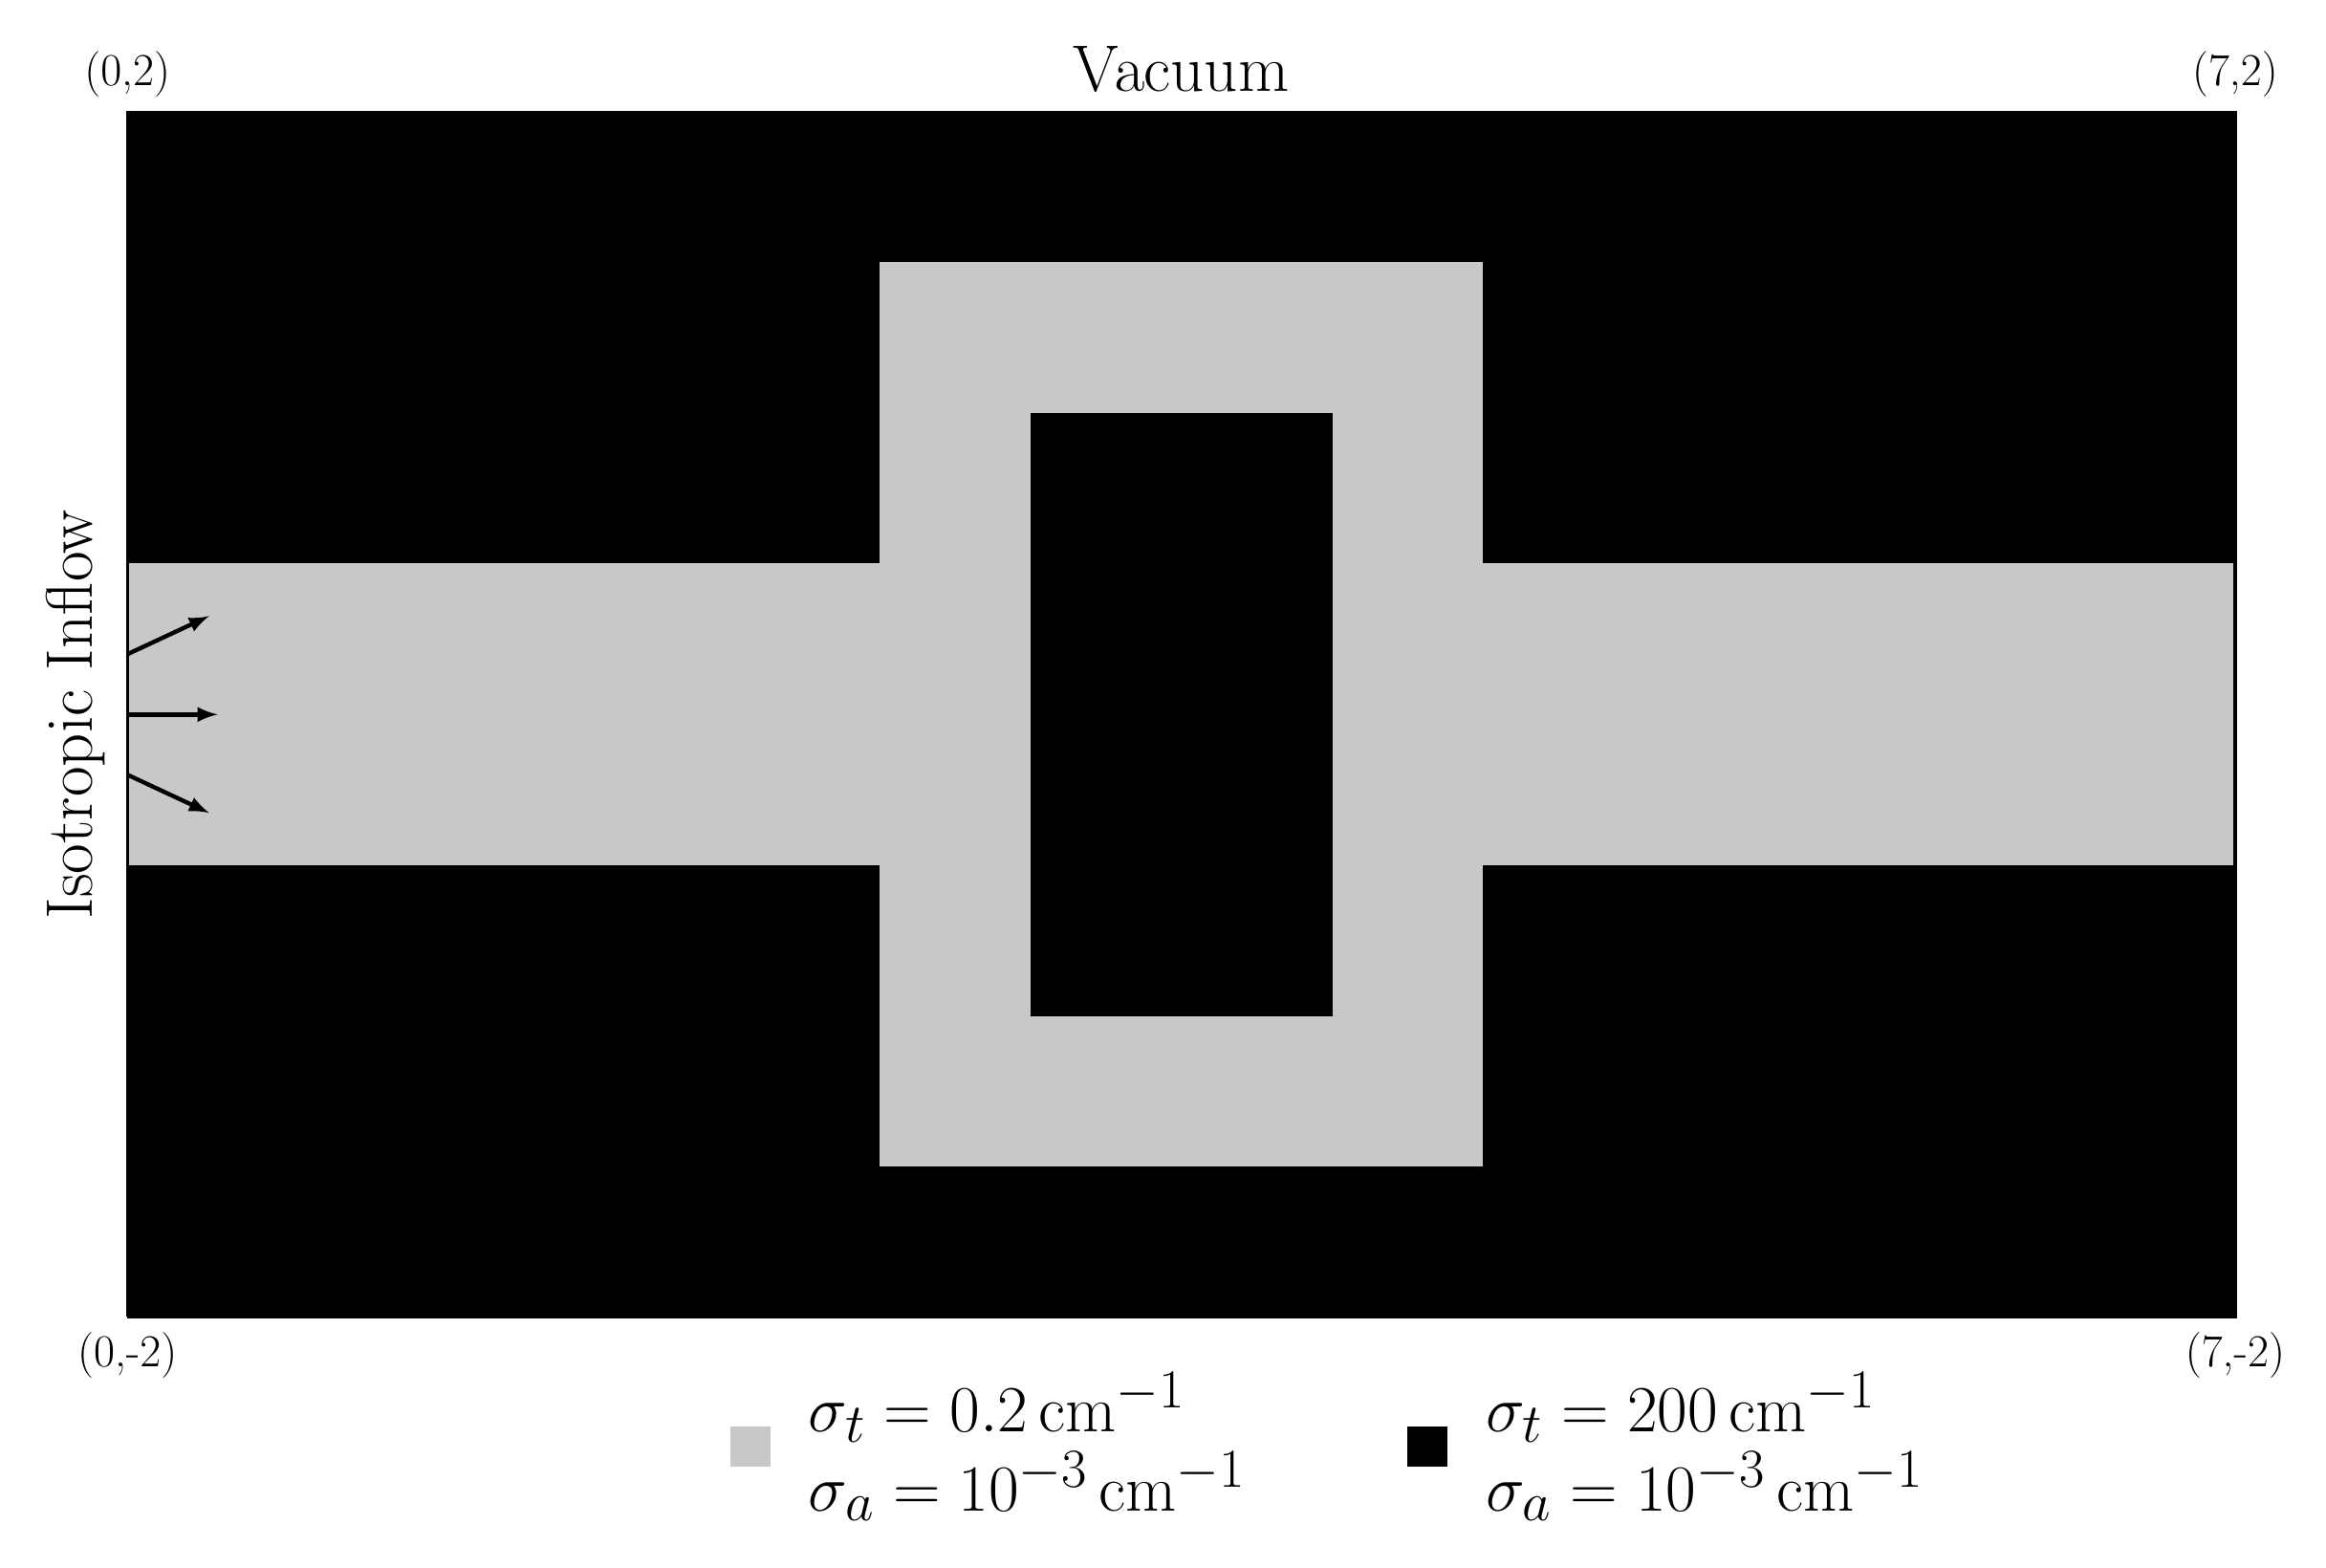
\begin{tikzpicture}[scale=4]
	\Huge
	\filldraw[founder] (0,-2) -- (7,-2) -- (7,2) -- (0,2) -- (0,-2); 
	\filldraw[calgold] (0,-.5) -- (2.5,-.5) -- (2.5,-1.5) -- (4.5,-1.5) -- (4.5,-.5) -- (7,-.5) -- (7,.5) -- (4.5,.5) -- (4.5,1.5) -- (2.5,1.5) -- (2.5,.5) -- (0,.5); 
	\filldraw[founder] (3,-1) -- (4,-1) -- (4,1) -- (3,1); 
	\draw[->, >=latex, ultra thick] (0,0) node[rotate=90, anchor=south] {Isotropic Inflow} -- +(0:3mm) ; 
	\draw[->, >=latex, ultra thick] (0,-.2) -- +(-25:3mm); 
	\draw[->, >=latex, ultra thick] (0,.2) -- +(25:3mm); 
	\LARGE
	\draw[very thick,black] (0,-2) node[below,black] {(0,-2)} -- (7,-2) node[below,black] {(7,-2)} -- (7,2) node[above,black] {(7,2)} -- (0,2) node[above,black] {(0,2)} -- (0,-2); 
	\Huge
	\node[above, anchor=south, black] at (3.5,2) {Vacuum}; 

	\node[rectangle, minimum size=5mm, fill=calgold, anchor=south west] (pipe) at (2,-2.5) {}; 
	\node[right=.5cm, text width=6cm] at (pipe) {$\sigma_t = \SI{0.2}{\per\cm}$\\ $\sigma_a = 10^{-3}\,\si{\per\cm}$}; 
	% \node[right=2mm, text width=3cm] at (pipe) {$\sigma_t = \SI{0.2}{\per\cm}$\\$\sigma_a = 10^{-3}\,\si{\per\cm}$}; 
	% \node[rectangle, minimum size=5mm, fill=founder, anchor=south west, right=3.25cm] (wall) at (pipe) {}; 
	% \node[right=2mm, text width=3cm] at (wall) {$\sigma_t = \SI{200}{\per\cm}$\\$\sigma_a = 10^{-3}\,\si{\per\cm}$}; 
	\node[rectangle, minimum size=5mm, fill=founder, anchor=south west] (wall) at (4.25,-2.5) {}; 
	\node[right=.5cm, text width=6cm] at (wall) {$\sigma_t = \SI{200}{\per\cm}$\\$\sigma_a = 10^{-3}\,\si{\per\cm}$}; 
\end{tikzpicture}
\end{document}